\documentclass{beamer}
\usepackage[ngerman]{babel}% Language
\usepackage{graphicx}
\usepackage{tikzsymbols}
\usetheme{Warsaw}
\makeatletter
\setbeamertemplate{title page}
{
\vbox{}
{\usebeamercolor[fg]{titlegraphic}\inserttitlegraphic\hfill\inserttitlegraphicii\par}
\begin{centering}
    \begin{beamercolorbox}[sep=8pt,center]{institute}
        \usebeamerfont{institute}\insertinstitute
    \end{beamercolorbox}
    \begin{beamercolorbox}[sep=8pt,center]{title}
        \usebeamerfont{title}\inserttitle\par%
        \ifx\insertsubtitle\@empty%
        \else%
        \vskip0.25em%
        {\usebeamerfont{subtitle}\usebeamercolor[fg]{subtitle}\insertsubtitle\par}%
        \fi
        %
    \end{beamercolorbox}%
    \vskip1em\par
    \begin{beamercolorbox}[sep=8pt,center]{date}
        \usebeamerfont{date}\insertdate
    \end{beamercolorbox}%\vskip0.5em
    \begin{beamercolorbox}[sep=8pt,center]{author}
        \usebeamerfont{author}\insertauthor
    \end{beamercolorbox}
\end{centering}
%\vfill
}
\author{Adrian Helberg, Rodrigo Ehlers}
\title{Intelligente Systeme Praktikum}
\subtitle{Aufgabe 2 - Lernen}
\date{\today}
\titlegraphic{
\includegraphics[height=1.5cm]{../haw_logo.png}}

%%% Blöcke
% RED
\newenvironment<>{red}[1]{
\setbeamercolor{block title}{fg=white,bg=red!75!black}
\begin{block}#2{#1}}{\end{block}}
% BLUE
\newenvironment<>{blue}[1]{
\setbeamercolor{block title}{fg=white,bg=blue!75!black}
\begin{block}#2{#1}}{\end{block}}
% LIGHTBLUE
\newenvironment<>{lightblue}[1]{
\setbeamercolor{block title}{fg=white,bg=blue!100!black}
\begin{block}#2{#1}}{\end{block}}
% YELLOW
\newenvironment<>{definition}[1]{
\setbeamercolor{block title}{fg=white,bg=green!75!black}
\begin{block}#2{#1}}{\end{block}}

\begin{document}

\begin{frame}[plain]
\maketitle
\end{frame}

\begin{frame}{Inhalt}
\tableofcontents
\end{frame}

\section{Thema}
\begin{frame}{Thema}
\begin{blue}{Beschreibung}
Handschrifterkennung mittels k\"unstlichem neuronalem Netz (KNN)
\end{blue}

\begin{lightblue}{\"Uberlegungen}
Wir ben\"otigen:
\begin{itemize}
\item \underline{Neuronales Netz}: Hier findet das Lernen statt
\item \underline{Lerndaten}: Datensatz, durch den das KNN lernt
\item \underline{Testdaten}: Validieren des KNN, Bestimmen der ''Genauigkeit''
\item Anwendungsdaten: M\"oglichkeit handgeschriebene Zahlen dem KNN zu ''\"ubergeben''
\end{itemize}
\end{lightblue}
\end{frame}

\section{Neuronale Netze}
\begin{frame}{Neuronale Netze - Allgemeine Beschreibung}
\begin{definition}{Definition}
Als neuronales Netz wird in den Neurowissenschaften eine beliebige Anzahl miteinander verbundener Neuronen bezeichnet, die als Teil eines Nervensystems einen Zusammenhang bilden, der einer bestimmten Funktion dienen soll
\end{definition}
\begin{red}{Eignet sich die Problemstellung?}
Eignet sich ein KNN \"uberhaupt f\"ur das L\"osen des Problems, oder l\"asst es sich auch durch das direkte Implementieren in einer Programmiersprache l\"osen?
\end{red}
\end{frame}

\begin{frame}{Neuronale Netze - \"Uberlegung}
\begin{lightblue}{Eignet sich die Problemstellung?}
Da sich das Erkennen von handschriftlichen Zeichen nicht direkt in einem Flussdiagramm ableiten l\"asst, und sich daher nicht direkt in einer Programmiersprache implementieren l\"asst, eignet sich ein Neuronales Netz gut f\"ur das Problem. Weiter eignet sich ein KNN besonders gut f\"ur ein Problem, das sich stetig ver\"andert und dessen L\"osung eine Anpassung verlangt
\end{lightblue}
\end{frame}

\begin{frame}{Neuronale Netze - Neuron}
\begin{center}
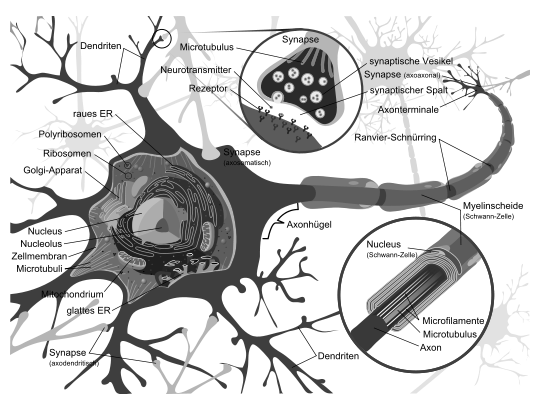
\includegraphics[height=6cm]{../Neuronenmodell.png}
\end{center}
\end{frame}

\begin{frame}{Neuronale Netze - Formales Neuron}
\begin{center}
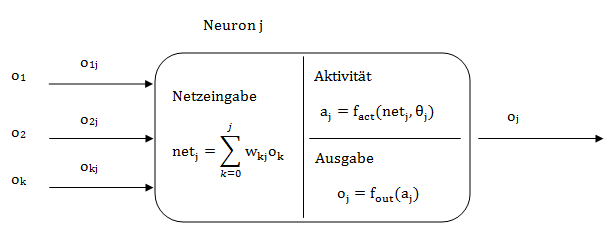
\includegraphics[height=2.8cm]{../Softwarebaustein_Neuron.png}
\begin{blue}{Beschreibung}
\begin{itemize}
\item Netzeingabe: Propagieren aller Eingabeinformationen mit den Gewichten der Verbindungen zu einer einzigen Netzeingabe
\item Aktivit\"at: Ermitteln eines Aktivierungszustands a\textsubscript{j} mittels Aktivierungsfunktion f\textsubscript{act}
\item Ausgabe: Weitergeben des Aktivierungszustands o\textsubscript{j}
\end{itemize}
\end{blue}
\end{center}
\end{frame}

\begin{frame}{Neuronale Netze - Lernprozess}
\begin{center}
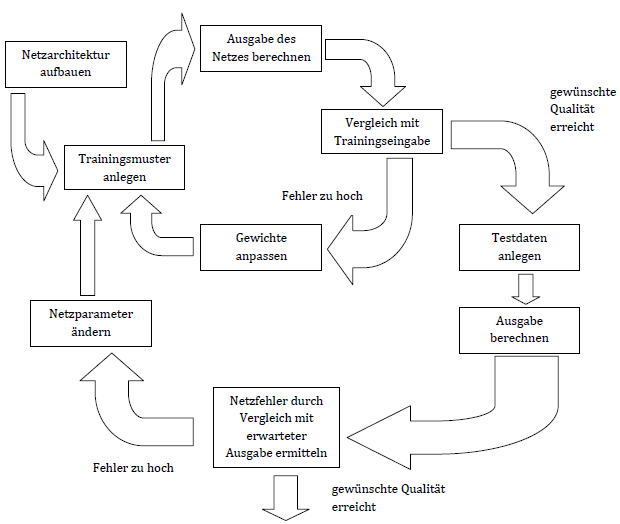
\includegraphics[height=6.5cm]{../Lernprozess.png}
\end{center}
\end{frame}

\begin{frame}{Neuronale Netze - Lernen}
\begin{lightblue}{Welche Lernmethode eignet sich gut?}
\"Uberwachtes, nicht \"uberwachtes oder best\"arkendes Lernen?
\end{lightblue}
\begin{blue}{L\"osung}
Die ''MNIST-Datenbank mit handgeschriebenen Ziffern'' stellt sowohl einen Datensatz mit potentiellen Lerndaten, als auch einen Datensatz zum Testen zur Verf\"ugung
\end{blue}
\end{frame}

\section{MNIST}
\begin{frame}{MNIST}
\begin{definition}{The MNIST database}
The MNIST database of handwritten digits, available from this page, has a training set of 60,000 examples, and a test set of 10,000 examples. It is a subset of a larger set available from NIST. The digits have been size-normalized and centered in a fixed-size image.
It is a good database for people who want to try learning techniques and pattern recognition methods on real-world data while spending minimal efforts on preprocessing and formatting.
\footnote[42]{\url{http://http://yann.lecun.com/exdb/mnist/}}
\end{definition}
\end{frame}

\section{Aktivierungsfunktion}
\begin{frame}{Aktivierungsfunktion}
\begin{blue}{Biologisches Vorbild}
\begin{itemize}
\item Biologische Neuronen arbeiten analog, d.h. sie k\"onnen auf kontinuierliche Schrittfolgen reagieren
\item Computer sind digitale Rechenmaschinen mit nur zwei Zuständen, 0 oder 1 (Quantencomputer ausgeschlossen \dSmiley )
\item K\"unstliche Neuronen müssen deshalb analoge Schwellwertfunktionen nachbilden
\end{itemize}
\end{blue}
\end{frame}

\begin{frame}{Aktivierungsfunktion}
\begin{definition}{Sigmoidfunktionen}
\begin{center}
Schwellwertfunktion / logistische Funktion 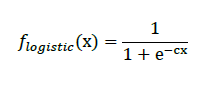
\includegraphics[height=1cm]{../Sigmoidfunktion.png}
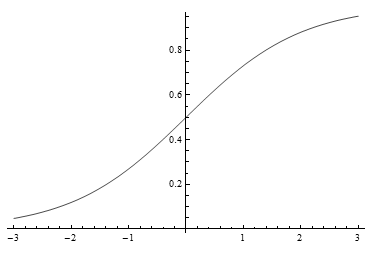
\includegraphics[height=4.2cm]{../Sigmoidfunktion_koordinatensystem.png}
\end{center}
\end{definition}
\end{frame}

\section{Lernregel}
\begin{frame}{Lernregel - Beschreibung}
Die Lernregel gestattet es, dass ein KNN durch eine gegebene Aufgabe (weitgehend) selbst\"andig aus Beispielen lernt
\begin{definition}{Die Lernregel bestimmt}
\begin{itemize}
\item die Entwicklung neuer Verbindungen
\item das Löschen existierender Verbindungen
\item die Modifikation der Stärke wi von Verbindungen
\item die Modifikation des Schwellenwertes von Neuronen
\item die Modifikation der Aktivierungs-, Propagierungs- oder Ausgabefunktion
\item die Entwicklung neuer Neuronen
\item das Löschen von Neuronen
\end{itemize}
\end{definition}
\end{frame}

\begin{frame}{Lernregel - \"Uberlegung}
\begin{lightblue}{\"Uberlegung}
Da wir eine nicht-lineare Aktivierungsfunktion gew\"ahlt haben, muss die
 Lernregel semilinear, d.h. monoton und differenzierbar, sein
\end{lightblue}
\begin{blue}{Backpropagation}
Die Backpropagation-Regel erf\"ullt die Kriterien
\end{blue}
\end{frame}

\begin{frame}{Lernregel - Backpropagation I}
\begin{center}
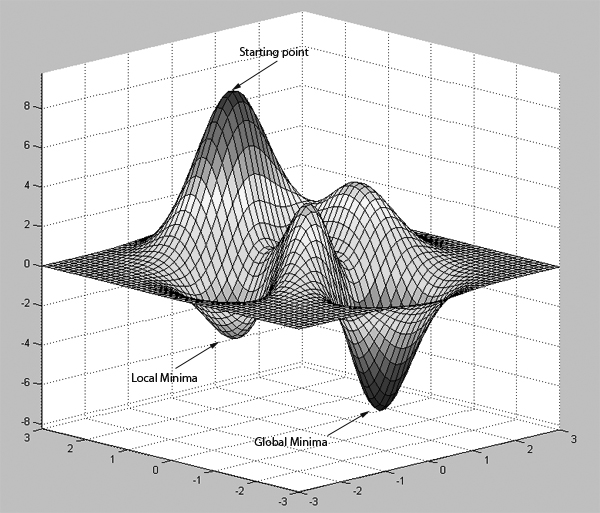
\includegraphics[height=6.5cm]{../Backpropagation.png}
\end{center}
\end{frame}

\begin{frame}{Lernregel - Backpropagation II}
\begin{definition}{Korrektur von Gewichten}
Die partielle erste Ableitung der Fehlerfunktion nach einer Gewichtsvariablen kann für die Korrektur dieses Gewichtes verwendet werden:
\begin{center}
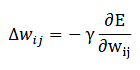
\includegraphics[height=1.4cm]{../Erste_ableitung_fehlerfunktion.png}
$\rightarrow$
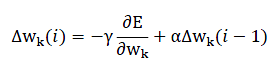
\includegraphics[height=1.4cm]{../Korrektur_gewicht.png}
\end{center}
Mit \textit{E} als m\"ogliche Fehlerkurve \textit{E(w\textsubscript{1}, w\textsubscript{2}) }f\"ur zwei Gewichte; Lernrate $\gamma$, als Grad der \"Anderung und Momentum $\alpha$
\end{definition}
\end{frame}

\section{Qualit\"at}
\begin{frame}{Qualit\"at}
\begin{blue}{Einfluss auf die Qualit\"at des Backpropagation-Lernverfahrens}
\begin{itemize}
\item Festlegung des Lernparameters $\gamma$
\item Wahl und Symmetrie der Initialisierungsgewichte
\item Anzahl der Neuronen
\end{itemize}
\end{blue}
\end{frame}

\begin{frame}{Qualit\"at - Belegungen I}
\begin{blue}{Lernparameter $\gamma$}
\begin{itemize}
\item Wird meist zwischen 0 und 1 festgelegt (in Ausnahmef\"allen kann dieser Wert aber auch h\"oher sein)
\item Es existieren keine Regeln, da der Parameter in Abh\"angigkeit von der Problemstellung und den Trainingsdaten gew\"ahlt wird
\end{itemize}
\end{blue}
\begin{lightblue}{Belegungen}
Durch ''Herumprobieren'' sollen passende Belegungen f\"ur $\gamma$ und die pseudo-zuf\"alligen Gewichte gefunden werden. Die Qualit\"at des Ergebnisses machen wir and der ''Genauigkeit'' (Accuracy) des neuronalen Netzes aus
\end{lightblue}
\end{frame}

\begin{frame}{Qualit\"at - Belegungen II}
\begin{blue}{Anzahl Neuronen}
Die Anzahl der Neuronen im Hidden-Layer sollte...
\begin{itemize}
\item zwischen der Anzahl an Input-Layer-Neuronen und der Anzahl an Output-Layer-Neuronen sein
\item 2/3 der Anzahl der Input-Layer-Neuronen + die Anzahl an Output-Layer-Neuronen sein
\item weniger als die doppelte Anzahl an Input-Layer-Neuronen sein
\end{itemize}
\end{blue}
\end{frame}

\begin{frame}{Tests - $\gamma$}
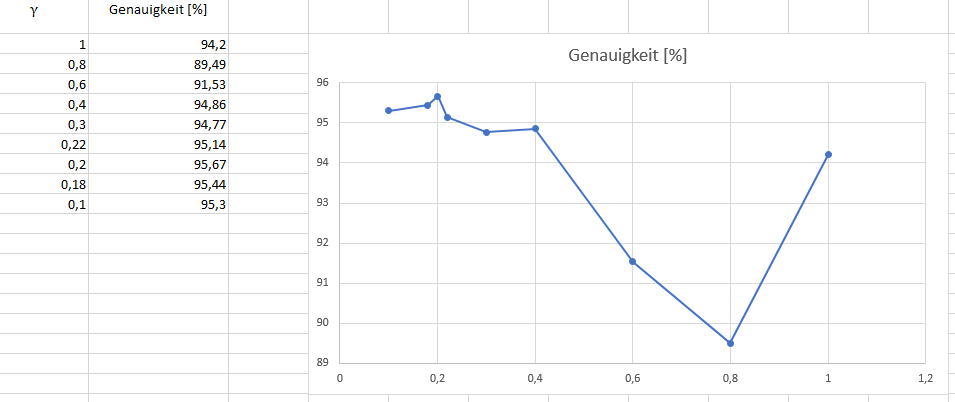
\includegraphics[height=5.5cm]{../Belegungen.png}
\end{frame}

\section{Fazit}
\begin{frame}{Fazit}
\begin{lightblue}{Fazit}
Wir haben nun alles, um eine Handschrifterkennung mittels neuronalem Netz in einer Programmiersprache (Java) umzusetzen
\end{lightblue}
\end{frame}

\end{document}